%This work is licensed under the Creative Commons
%Attribution-ShareAlike 4.0 International License. To view a copy of
%this license, visit http://creativecommons.org/licenses/by-sa/4.0/ or
%send a letter to Creative Commons, PO Box 1866, Mountain View, CA
%94042, USA.

%This work is licensed under the Creative Commons
%Attribution-ShareAlike 4.0 International License. To view a copy of
%this license, visit http://creativecommons.org/licenses/by-sa/4.0/ or
%send a letter to Creative Commons, PO Box 1866, Mountain View, CA
%94042, USA.

%\documentclass[gray,handout, pdftex, 11pt]{beamer}
%\documentclass[handout, pdftex, 11pt]{beamer}

\documentclass[pdftex, 11pt]{beamer}

\usepackage[utf8]{inputenc}
\usepackage[T1]{fontenc}
\usepackage{lmodern}
%\usepackage[italian]{babel}
\usepackage{graphicx}
\usepackage{listings}
\usepackage{microtype}
\usepackage{acronym}
\usepackage{array}
\usepackage{tikz}
\usetikzlibrary{shapes, chains, scopes, shadows, positioning, arrows,
  decorations.pathmorphing, calc}

\colorlet{c1}{green!20}
\colorlet{c2}{blue!10}
\colorlet{drawColor}{black!50}
\colorlet{commentColor}{green!70!black!90}

\tikzstyle{oval}=[ellipse, align=center, drop shadow, draw=drawColor, fill=white]
\tikzstyle{rect}=[rectangle, rounded corners=2pt, align=center, drop
shadow, draw=drawColor, fill=white]
\tikzstyle{comment}=[text=commentColor,font=\itshape]
\tikzstyle{textLab}=[]
\tikzstyle{arrow}=[->, very thick, >=stealth', draw=black!80]
\tikzstyle{darrow}=[->, dash pattern=on 3pt off2pt, very thick, >=stealth', draw=black!80]
\tikzstyle{fStartEnd}=[ellipse, align=center, drop shadow, draw=drawColor, fill=white]
\tikzstyle{fInput}=[trapezium, trapezium left angle=70, trapezium right angle=110,
align=center, drop shadow, draw=drawColor, fill=white]
\tikzstyle{fProcess}=[rectangle, align=center, drop shadow, draw=drawColor, fill=white]
\tikzstyle{fSelection}=[diamond, shape aspect=3, align=center, drop
shadow, draw=drawColor, fill=white]
\tikzstyle{fOutput}=[tape, tape bend top=none, align=center, drop shadow, draw=drawColor, fill=white]
\tikzstyle{mem}=[rectangle, align=center, draw=drawColor, fill=white]
\tikzstyle{clo}=[cloud, aspect=2, align=center, drop shadow, draw=drawColor, fill=white]

\lstdefinestyle{customc}{
   language=C,
   % basicstyle=\small\ttfamily\bfseries,
   basicstyle=\ttfamily,
   keywordstyle=\color{blue}\ttfamily,
   stringstyle=\color{red}\ttfamily,
   commentstyle=\color{green}\ttfamily,
   morecomment=[l][\color{magenta}]{\#},
   % breaklines=false,
    breaklines=true, breakatwhitespace=false,
   frameround=fttt,
   frame=trBL,
   backgroundcolor=\color{yellow!20},
   numbers=left,
   stepnumber=1,    
   firstnumber=1,
   numberfirstline=true,
   numberstyle=\tiny\color{black!50},
   xleftmargin=2em,
   framexleftmargin=1.5em
   % linewidth=8cm,
}

\lstnewenvironment{cblock}[1][]
{
  \lstset{
    style=customc,
    #1
  }
}{}

\newcommand{\cfile}[2][]{
  \lstinputlisting[style=customc, #1]{#2}
}

\definecolor{links}{HTML}{2A1B81}
\hypersetup{colorlinks,linkcolor=links,urlcolor=links}

\definecolor{links}{HTML}{2A1B81}
\hypersetup{colorlinks,linkcolor=,urlcolor=links}


\mode<presentation>{
  %-------------------------1
  \usetheme{Boadilla}
  \usecolortheme{beaver}
  %-------------------------1
  %-------------------------2
  %\usetheme{Goettingen}
  %\usecolortheme{sidebartab}
  %-------------------------2
  %\useoutertheme[right]{sidebar}
  %\usefonttheme{default}
  \setbeamercovered{transparent}
  %\setbeameroption{show notes on second screen=right}
  \setbeamertemplate{navigation symbols}{}
  \setbeamertemplate{footline}{}

  \bibliographystyle{abbrv}  
  %\renewcommand\bibfont{\scriptsize}
  \setbeamertemplate{bibliography item}{\textbullet}
  \setbeamertemplate{itemize item}{\checkmark}
  \setbeamertemplate{itemize subitem}{-}
  \setbeamertemplate{enumerate items}[default]
  \setbeamertemplate{sections/subsections in toc}[square]
}

\subtitle{Logical Computational Thinking}
\institute[Tecnológico de Monterrey]{
  
\includegraphics[width=5cm]{img/logoTEC.jpg}\\[5mm]
  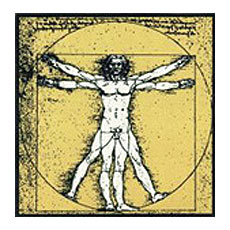
\includegraphics[width=1cm]{img/logoLEO.jpg}
  Scuola Leonardo Da Vinci (Firenze)
}

\author[Stefano Martina]{
  %\\[0.2cm]
  \textbf{Stefano MARTINA}\\
  {\small stefano.martina@gmail.com}
}

\titlegraphic{\tiny
  \href{http://creativecommons.org/licenses/by-sa/4.0/}{
\includegraphics[width=1cm]{img/logoCC.png}}
  This work is licensed under a
  \href{http://creativecommons.org/licenses/by-sa/4.0/}{Creative
    Commons Attribution-ShareAlike 4.0 International License}.}


\title[Lesson 1]{\textbf{Lesson 1 - Introduction and algorithms}}
\date[7/9/15]{\flushright 7 September 2015}

\begin{document}

\begin{frame}[plain]
  \titlepage
\end{frame}

\begin{frame}
  \frametitle{Material}
  \begin{block}{Material}
    all the material will be available at \url{https://github.com/trianam/courseLCT1516}
  \end{block}
  \pause
  \begin{block}{Book}
    \url{https://www.dropbox.com/s/umx65z3m9bnm6xj/Metodologia_de_la_programacion__3ra_Edicion_-_Osvaldo_Cairo_Battistutti.pdf}
  \end{block}
\end{frame}

\begin{frame}
  \frametitle{Evaluation}
    \begin{itemize}
  \item You will be evaluated continuously along the lectures
    \begin{itemize}
    \item exercises
    \item questions
    \item etc...
    \end{itemize}
  \item and with exams
    \begin{itemize}
    \item 2 partials (maybe 1)
    \item 1 final (project)
    \end{itemize}
  \end{itemize}
\end{frame}

\begin{frame}
  \frametitle{History}
  \begin{itemize}
  \item classical age and middle ages: \alert{algorisms} \\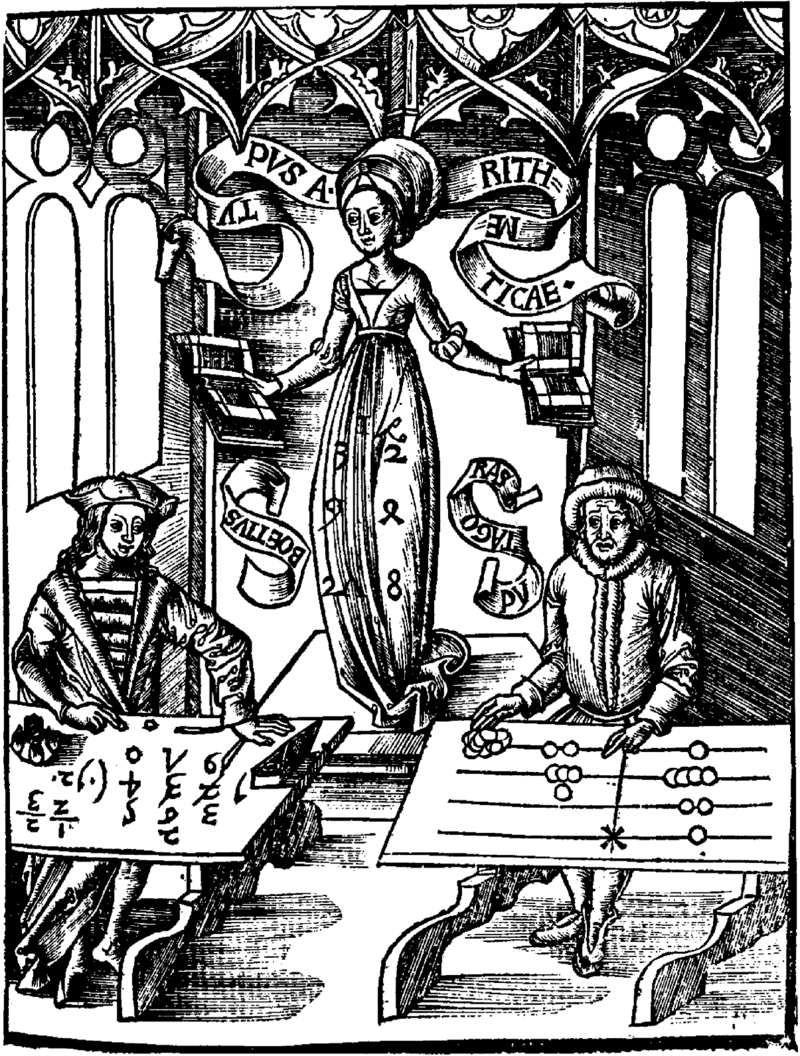
\includegraphics[width=2cm]{algorism.png}
  \item 1833-1842: \alert{Analytical engine} of Charles
    Babbage (Ada Byron) \\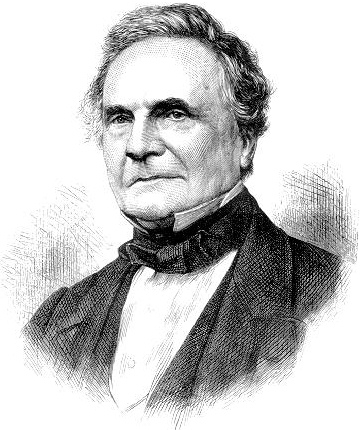
\includegraphics[width=2cm]{babbage.jpg}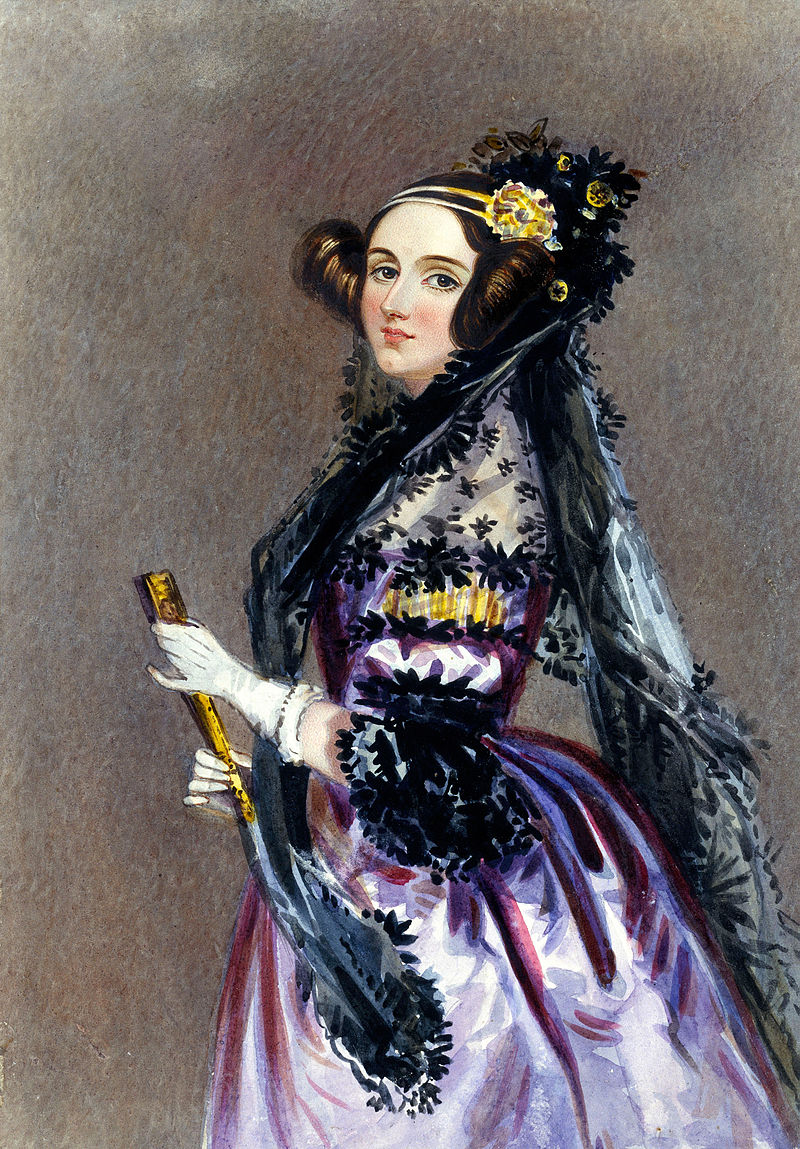
\includegraphics[width=2cm]{lovelace.jpg}
  \end{itemize}
\end{frame}

\begin{frame}
  \frametitle{History}
  \begin{itemize}
  \item before and during WW2: first modern computers (single purpose,
    programmable), \alert{Turing} studies \\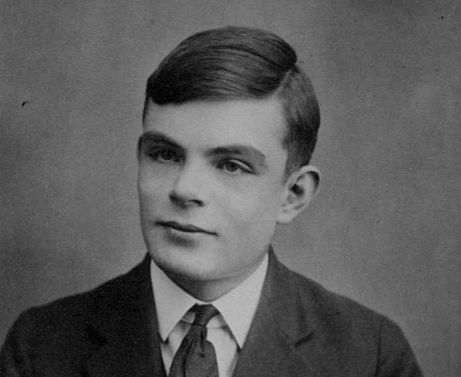
\includegraphics[width=2cm]{turing.jpg}
  \item 1946: \alert{ENIAC} (general purpose) \\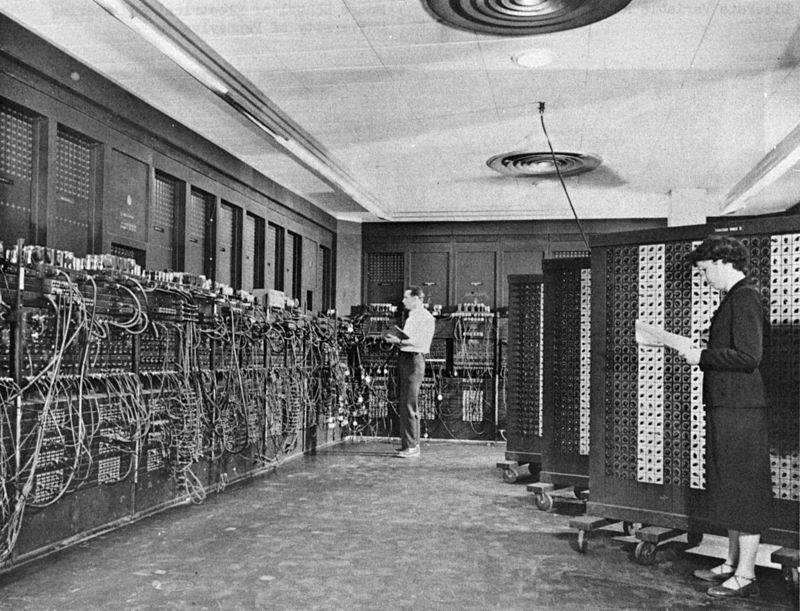
\includegraphics[width=2cm]{eniac.jpg}
  \item 1951: \alert{EDVAC}, Von Neumann architecture \\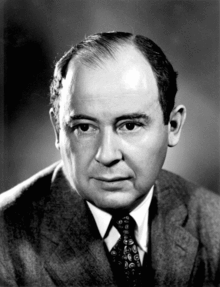
\includegraphics[width=2cm]{vonNeumann.png}
  \end{itemize}
\end{frame}

\begin{frame}
  \frametitle{Computer architecture (Von Neumann)}
  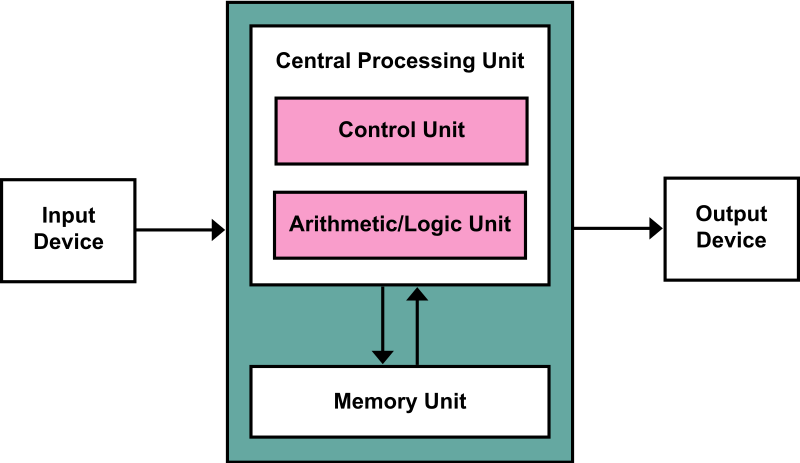
\includegraphics[width=\textwidth]{vonNeumannArchitecture.png}
\end{frame}

\begin{frame}
  \frametitle{Input/Output}
  \begin{block}{Input devices}
    \begin{itemize}
    \item Keyboard
    \item Mouse
    \end{itemize}
  \end{block}
  \pause
  \begin{block}{Output devices}
    \begin{itemize}
    \item Screen
    \item Printer
    \end{itemize}
  \end{block}
  \pause
  \begin{block}{Input/output devices}
    \begin{itemize}
    \item Hard disk
    \item Network card
    \end{itemize}
  \end{block}
\end{frame}

\begin{frame}
  \frametitle{Algorithms}
  \begin{itemize}
  \item a series of ordered \alert{steps}
  \item with the goal of performing a \alert{task}
  \end{itemize}
  \pause
  \begin{block}{Examples}
    \begin{itemize}
    \item a recipe
    \item an algebraic procedure
    \end{itemize}
  \end{block}
\end{frame}

\begin{frame}
  \frametitle{Program}
  \begin{itemize}
  \item An implementation of an \alert{algorithm} in a certain
    \alert{programming language} (software)
    \pause
  \item A program can be \alert{executed} by a \alert{machine}
    (hardware)
    \pause
  \item Often a program need to be \alert{compiled} before the
    execution (\alert{transformed} in something understandable from the
    machine)
  \end{itemize}
\end{frame}

\begin{frame}
  \frametitle{Literary comparison}
  \begin{description}
  \item[Algorithm:] the history \\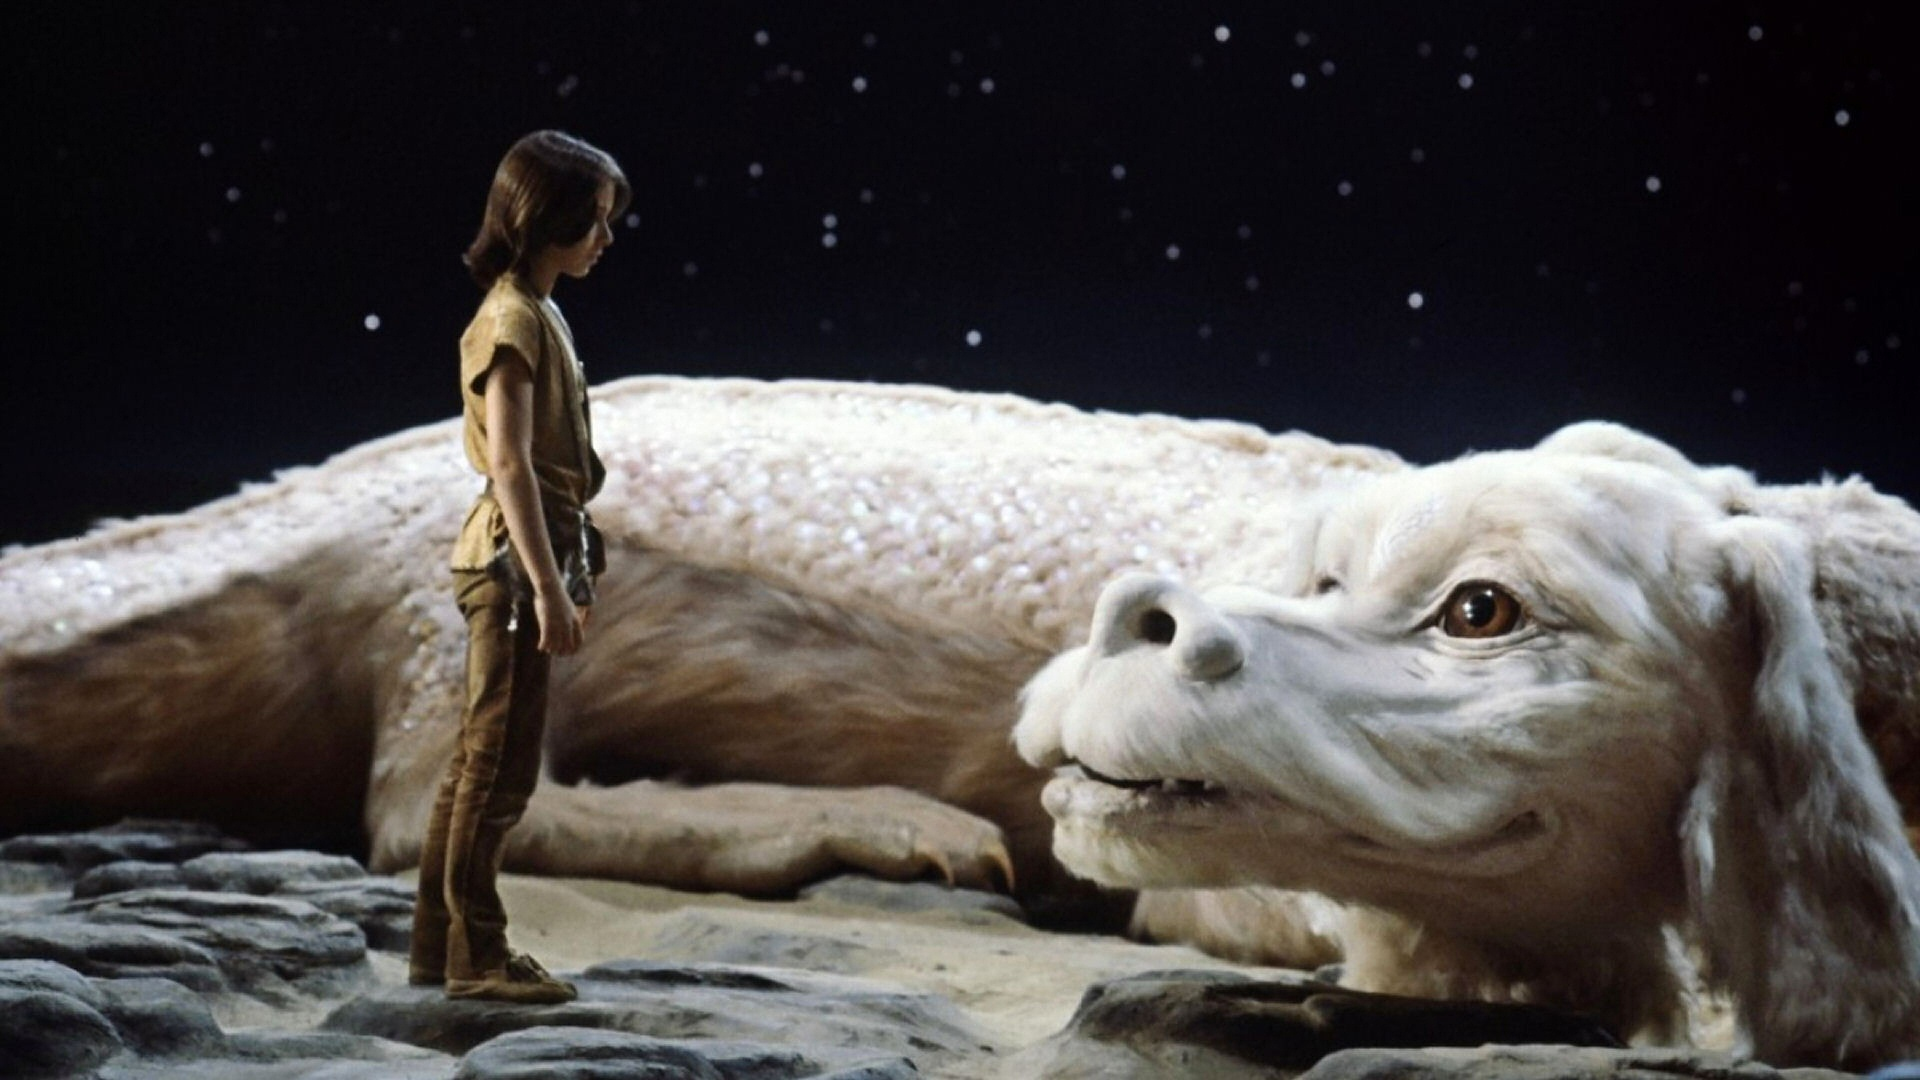
\includegraphics[width=3cm]{neverEndingStory1.jpeg}
  \item[Program:] the text\\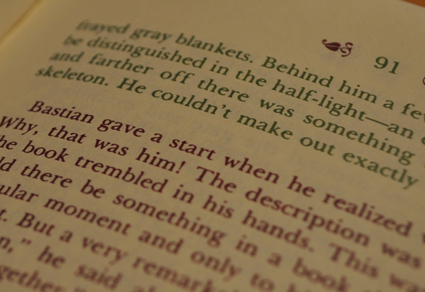
\includegraphics[width=3cm]{neverEndingStory2.jpeg}
  \item[Hardware:] the book\\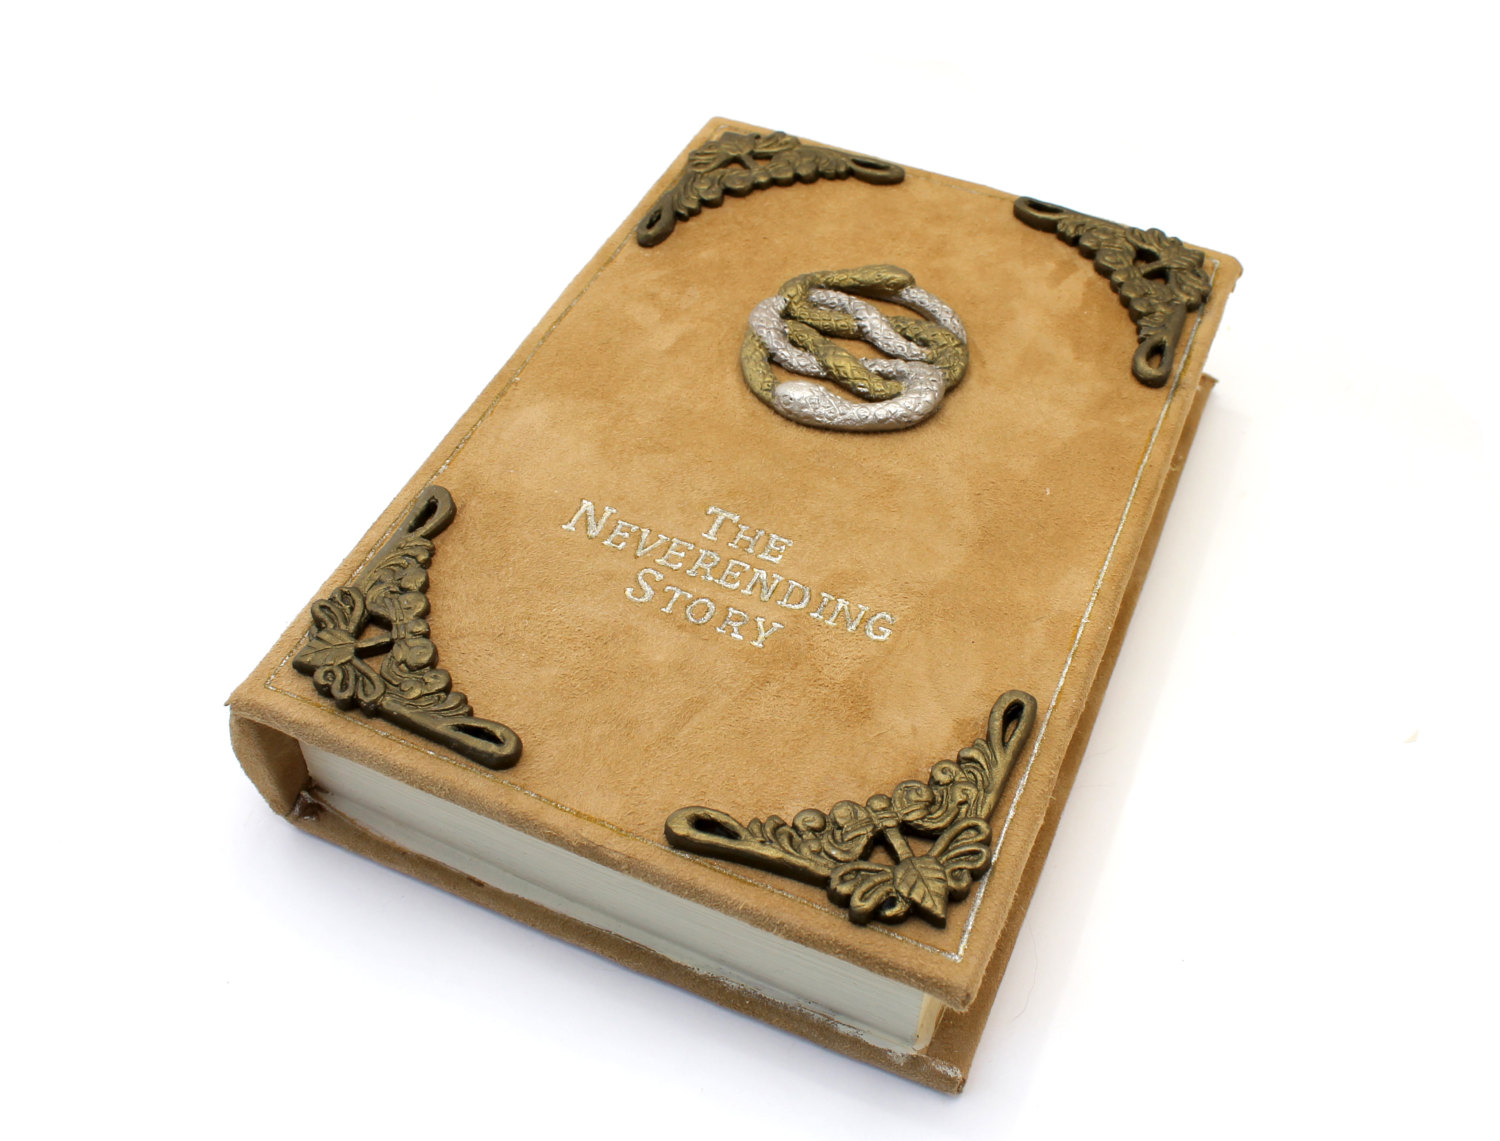
\includegraphics[width=3cm]{neverEndingStory3.jpeg}
  \end{description}
\end{frame}

\begin{frame}
  \frametitle{How to develop a program}
  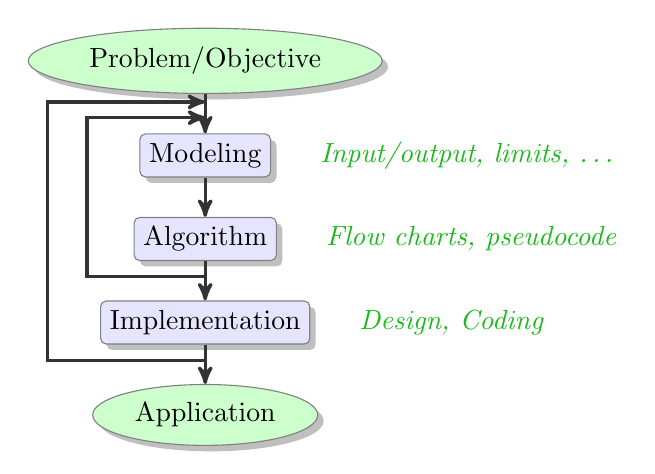
\begin{tikzpicture}[node distance=5mm]
    \node (realProb) [oval, fill=c1] {Problem/Objective};
    \pause
    \node (model) [rect, fill=c2, below=of realProb] {Modeling};
    \node [comment, right=of model] {Input/output, limits, \dots};
    \draw [arrow] (realProb) -- (model);
    \pause
    \node (algorithm) [rect, fill=c2, below=of model] {Algorithm};
    \node [comment, right=of algorithm] {Flow charts, pseudocode};
    \draw [arrow] (model) -- (algorithm);
    \pause
    \node (implementation) [rect, fill=c2, below=of algorithm] {Implementation};
    \node [comment, right=of implementation] {Design, Coding};
    \draw [arrow] (algorithm) -- (implementation);
    \pause
    \node (application) [oval, fill=c1, below=of implementation] {Application};
    \draw [arrow] (implementation) -- (application);
    \pause
    \draw [arrow] ($ (implementation.south) + (0,-2mm) $) -- ++(-20mm,0) |- ($ (model.north) + (0,4mm) $);
    \draw [arrow] ($ (algorithm.south) + (0,-2mm) $) -- ++(-15mm,0) |- ($ (model.north) + (0,2mm) $);
  \end{tikzpicture}
\end{frame}

\begin{frame}
  \frametitle{Model}
  \begin{enumerate}
  \item \alert{Analyze} the problem or the required objective
  \item \alert{Contextualize} in an algorithmic way
  \item \alert{Identify} the key concept/mechanisms, how to divide the
    problem in subproblems
  \end{enumerate}
\end{frame}

\begin{frame}
  \frametitle{Algorithm}
  \begin{block}{Concept}
    Use techniques to ``put down'' ideas on how to resolve the problem.
  \end{block}
  \pause
  \begin{enumerate}
  \item Flow charts
  \item Pseudocode
  \end{enumerate}
  \pause
  \begin{block}{Implementation}
    \alert{Transform} the algorithm in code
  \end{block}
\end{frame}

\begin{frame}
  \frametitle{Flow charts}
  \begin{block}{Definition}
    \alert{Symbols} with different meanings and descriptions,
    \alert{combined} with the logic of the flow along the time
  \end{block}
  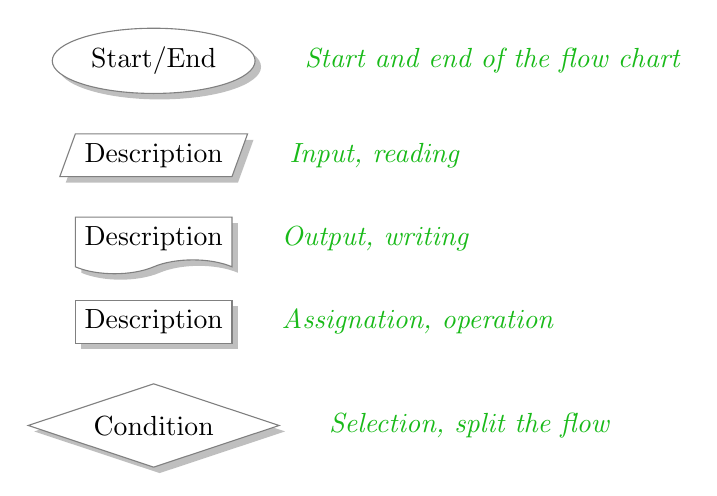
\begin{tikzpicture}[node distance=5mm]
    \node (startEnd) [fStartEnd] {Start/End};
    \node [comment, right=of startEnd] {Start and end of the flow chart};
    \node (input) [fInput, below=of startEnd] {Description};
    \node [comment, right=of input] {Input, reading};
    \node (output) [fOutput, below=of input] {Description};
    \node [comment, right=of output] {Output, writing};
    \node (process) [fProcess, below=of output] {Description};
    \node [comment, right=of process] {Assignation, operation};
    \node (selection) [fSelection, below=of process] {Condition};
    \node [comment, right=of selection] {Selection, split the flow};
  \end{tikzpicture}
\end{frame}

\begin{frame}
  \frametitle{Data types}
  \begin{block}{Data type}
    is the mean how the data is stored and manipulated
  \end{block}
  \begin{enumerate}
  \item \alert{Simple} represent single values
    \begin{itemize}
    \item boolean
    \item integer number
    \item floating point number (real number approximation)
    \item alfanumeric character
    \end{itemize}
  \item \alert{Structured} composed of multiple values
    \begin{itemize}
    \item string of characters
    \item array of values
    \item \dots
    \end{itemize}
  \end{enumerate}
  \pause
  All the data types have specific \alert{limits} (depending of the
  programming language)
\end{frame}

\begin{frame}
  \frametitle{Variables and costants}
  \begin{center}
    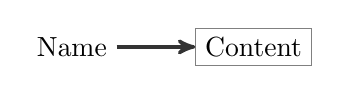
\begin{tikzpicture}
      \node (name) [textLab] {Name};
      \node (mem) [mem, right=of name] {Content};
      \draw [arrow] (name) -- (mem);
    \end{tikzpicture}    
  \end{center}
  \begin{block}{Variable}
    \begin{itemize}
    \item A name associated with a data type
    \item Use a certain amount of memory (specific to the data type)
    \item The content \alert{can} be modified
    \end{itemize}
  \end{block}
  \pause
  \begin{block}{Constant}
    \begin{itemize}
    \item A name associated with a data type
    \item Use a certain amount of memory (specific to the data type)
    \item The content \alert{can't} be modified
    \end{itemize}
  \end{block}
\end{frame}

\begin{frame}
  \frametitle{Example 1}
  \begin{block}{Problem}
    Given two integer \alert{A} and \alert{B}, calculate the sum
    \alert{A+B} and return it
  \end{block}
  \pause
  \begin{center}
    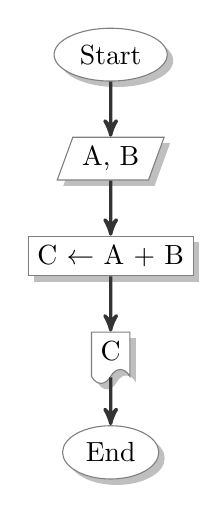
\begin{tikzpicture}[node distance=7mm]
      \node(start) [fStartEnd] {Start};
      \node(input) [fInput, below=of start] {A, B};
      \draw [arrow] (start) -- (input);
      \node(op) [fProcess, below=of input] {C $\leftarrow$ A + B};
      \draw [arrow] (input) -- (op);
      \node(output) [fOutput, below=of op] {C};
      \draw [arrow] (op) -- (output);
      \node(end) [fStartEnd, below=of output] {End};
      \draw [arrow] (output) -- (end);
    \end{tikzpicture}
  \end{center}
\end{frame}

\begin{frame}
  \frametitle{Example 2}
  \begin{block}{Problem}
    Given an integer \alert{A}, evaluate it's evenness value, and
    return \alert{true} if A is even, and \alert{false} if is odd
  \end{block}
  \pause
  \begin{center}
    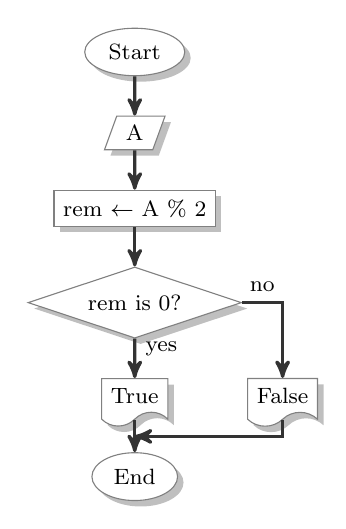
\begin{tikzpicture}[node distance=5mm, font=\footnotesize, auto]
      \node(start) [fStartEnd] {Start};
      \node(input) [fInput, below=of start] {A};
      \draw [arrow] (start) -- (input);
      \node(op) [fProcess, below=of input] {rem $\leftarrow$  A \% 2};
      \draw [arrow] (input) -- (op);
      \node(selection) [fSelection, below=of op] {rem is 0?};
      \draw [arrow] (op) -- (selection);
      \node(outputT) [fOutput, below=of selection] {True};
      \draw [arrow] (selection) -- node [near start] {yes} (outputT);
      \node(outputF) [fOutput, right=10mm of outputT] {False};
      \draw [arrow] (selection) -| node [near start] {no} (outputF);
      \node(end) [fStartEnd, below=of outputT] {End};
      \draw [arrow] (outputT) -- (end);
      \draw [arrow] (outputF) |- ($ (end.north) + (0,2mm) $);
    \end{tikzpicture}
  \end{center}
\end{frame}

\begin{frame}
  \frametitle{Exercise 1}
  \begin{block}{Problem}
    Given the reals \alert{$A$}, \alert{$B$}, and \alert{$C$} ($A$ is
    $\neq 0$), calculate the
    solutions \alert{$x_1$} and \alert{$x_2$} of the equation
    \alert{$Ax^2+Bx+C=0$} and return them. If the equation doesn't has
    solutions (real solutions), return \alert{$x_1=0$} and \alert{$x_2=0$}.
  \end{block}
  \pause
  Remember:
  \begin{enumerate}
  \item \alert{$\Delta$}$= B^2-4AC$
  \item if $\Delta \geq 0$ the solutions are:
    \begin{description}
    \item[\alert{$x_1$}]$=\frac{-B+\sqrt{\Delta}}{2A}$
    \item[\alert{$x_2$}]$=\frac{-B-\sqrt{\Delta}}{2A}$
    \end{description}
  \end{enumerate}
\end{frame}

\begin{frame}
  \frametitle{Exercise 2}
  \begin{block}{Problem}
    We have a parking with a limited number of 50 places. We also have
    two sensors that notify the passage of a car, one in the entrance
    and one in the exit. We want to put a semaphore in the entrance
    that is red when the parking is full and green when it isn't. 
  \end{block}
  \pause
  \begin{enumerate}
  \item Make a proper model, identify the different parts of the application
  \item Make a flow chart for each part
  \end{enumerate}
\end{frame}
\end{document}